\section{Design Option Structuring} \label{ch:design}
This chapter gives an overview of initial design concept selection, focusing on the different missions aspects of XXX. This concept generation is done systematically by means of a \gls{dot} for each of the aspects. Combination of the different trees then yields a number of final concepts. The next phase is eliminating clearly unfeasible or undevelopable concepts. The chapter commences with a \gls{dot} for each of the mission aspects in subsequent sections, including eliminating unfeasible concepts.

\subsection{Deceleration mechanism}
Deceleration can be performed by purely aerodynamic forces exerted by the local atmosphere, as used in the \gls{irve} missions (see Table \ref{tab:hiadcomparison}), primarily by a propulsive force (retro-propulsion) or a hybrid configuration featuring both, as used in for example the Apollo entry vehicles. Aerodynamic deceleration reduces the $\Delta V$ required by propulsion and is hence preferable to propulsive deceleration, i.e. retro-propulsion, through a decrease of the required entry mass by limiting required propellant to be taken on board. A feasibility study of \gls{nasa} indicates that pure propulsion is unfeasible by the large amounts of propellant mass required \cite{Cianciolo2010}. Moreover, by means of Tsiolkovsky's rocket equation it can be shown that a velocity increment of 7 $[km/s]$ is unattainable while keeping deceleration mechanism mass below 10 percent of initial mass for conventional effective exhaust velocities \cite{Wertz2011}. Figure \ref{fig:dotdelmech} gives the \gls{dot} for the deceleration mechanism.

Other options are un(der)developed: studies on their application for (re-)entry have not been found nor have these been considered in feasibility studies by \gls{nasa}, predominantly the extensive studies of Cianciolo et al \cite{Cianciolo2010}. As such, while these options may be worth revisiting in the future, their current state of development does not allow for implementation in a (re-)entry vehicle.

\begin{figure}[H]
\centering
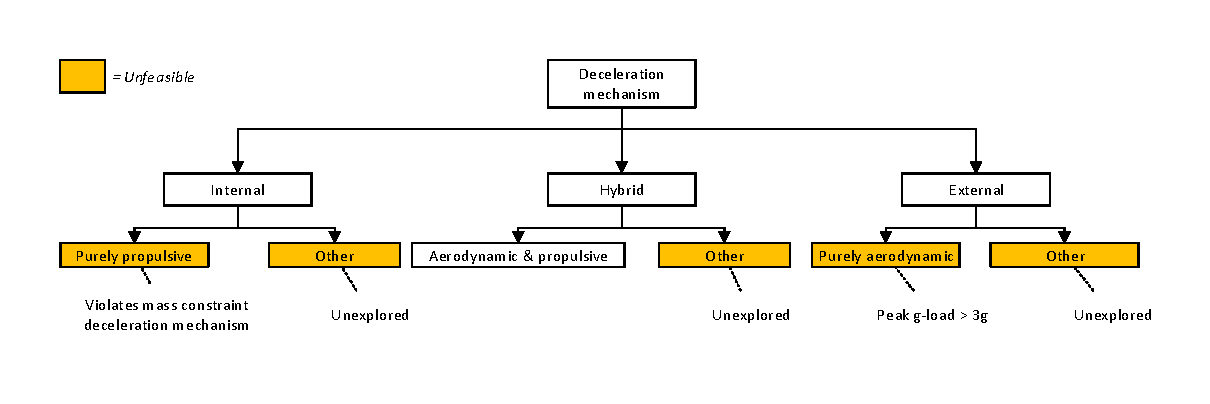
\includegraphics[width = 0.85\textwidth]{Figure/DOT_decelerationmechanism.pdf}
\caption{Design Option Tree for entry vehicle deceleration mechanism}
\label{fig:dotdelmech}
\end{figure}

\subsection{Configuration of aerodynamic deceleration}
The configuration of the aerodynamic deceleration mechanism can be subdivided into inflatable and non-inflatable systems. For non-inflatable systems an AND subdivision can be made. A blunt or pointed body can be considered and at the same time this structure may be deployable or undependable. Pointed bodies will not be considered since the attached shock will cause excessive aerodynamic heating \cite{} making this concept unfeasible. The blunt body may further be subdivided into lifting and non lifting bodies. Lifting bodies follow directly from the shape of the entry vehicle such as for example seen in the SpaceShuttle. Geometrically symmetric bodies may also feature a lifting component by featuring \gls{cg} located away from the symmetry axis. This \gls{cg} offset is sometimes also actively used for control purposes\cite{Dillman2012} as is also explained in section \ref{sec:DOTcontrol}. 


\begin{figure}[H]
\centering
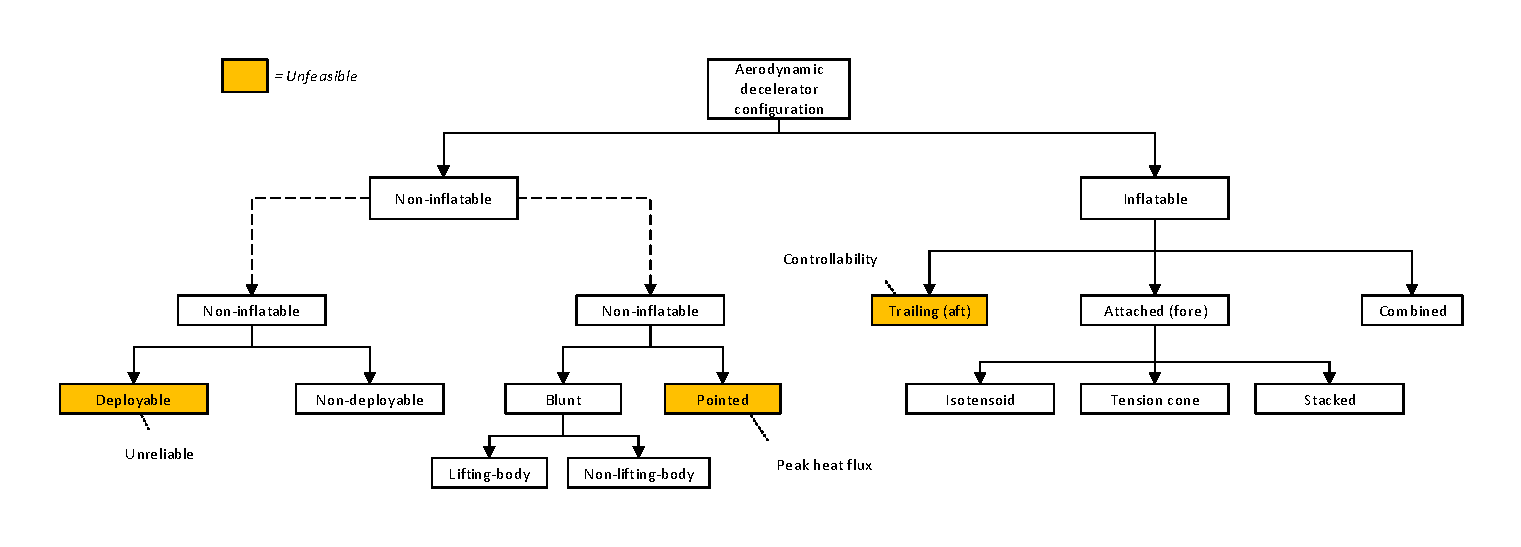
\includegraphics[width = 0.85\textwidth]{Figure/DOT_configuration.pdf}
\caption{Design Option Tree for entry vehicle deceleration mechanism}
\label{fig:dotdelconfg}
\end{figure}

\subsection{Trajectory control} \label{sec:DOTcontrol}


%\subsection{Inflation system}
%As mentioned in Chapter \ref{cha:litreview}, inflation can be performed either with (ram-air) or without use of the atmosphere. A third option is the use of both (hybrid), thereby featuring ram-air inlets as well as internal gas storage and feed systems. In terms of the medium used for inflation, conventionally nitrogen gas is used. An alternative would be hydrazine gas, as explained in Chapter \ref{cha:litreview}.
